% gjilguid2e.tex
% V2.0 released 1998 December 18
% V2.1 released 2003 October 7 -- Gregor Hutton, updated the web address for the style files.

%\documentclass[extra,mreferee]{gji}
\documentclass[extra]{gji}
\usepackage{timet}

%Extra packages
\usepackage{graphicx}
\usepackage{amsmath}

\title[Gravity anomaly or gravity disturbance?]
      {Should geophysicists use gravity anomaly or gravity disturbance?}
      
\author[Hallam et al.]
{Kristoffer A. T. Hallam$^{1}$\thanks{Emails: kristoffer.hallam@gmail.com,
vanderlei@on.br}, Vanderlei C. Oliveira Jr$^1$,
Val\'{e}ria C. F. Barbosa$^1$ \linebreak and Leonardo Uieda$^2$ \\
$^1$ Department of Geophysics, Observat\'{o}rio Nacional, Rio de Janeiro, Brazil \\
$^2$ Department of Geology and Geophysics, University of Hawaii, Manoa, USA
}

\date{Received 2018 Month XX; in original form 2018 Month XX}
\pagerange{\pageref{firstpage}--\pageref{lastpage}}
\volume{XXX}
\pubyear{2018}

%\def\LaTeX{L\kern-.36em\raise.3ex\hbox{{\small A}}\kern-.15em
%    T\kern-.1667em\lower.7ex\hbox{E}\kern-.125emX}
%\def\LATeX{L\kern-.36em\raise.3ex\hbox{{\Large A}}\kern-.15em
%    T\kern-.1667em\lower.7ex\hbox{E}\kern-.125emX}
% Authors with AMS fonts and mssymb.tex can comment out the following
% line to get the correct symbol for Geophysical Journal International.
\let\leqslant=\leq

\newtheorem{theorem}{Theorem}[section]

\begin{document}

\label{firstpage}

\maketitle


\begin{summary}
 In applied geophysics, the gravity anomaly has long been used for representing the
 gravitational effect produced by gravity sources, which are defined as the density
 contrasts between the internal density distribution of the Earth and the normal Earth.
 The gravity anomaly is defined by the difference between the gravity (produced by the
 Earth) on the Geoid and the normal gravity (produced by the normal Earth)
 on reference ellipsoid, both at the same geodetic latitude and longitude.
 Because these quantities are not defined at the same point, 
 the gravity anomaly does not represent the gravitational effect due to the gravity
 sources and, consequently, cannot be considered a harmonic function.
 On the contrary, the gravity disturbance is defined by the difference between
 the gravity and normal gravity at the same point. Consequently, the centrifugal 
 effects can be neglected, the gravity disturbance can be considered a harmonic 
 function representing the gravitational effect due to the gravity sources and then 
 it satisfies the premise behind most of the processing techniques of potential-field
 data (e.g., upward/downward continuations). Then, rigorously, the gravity disturbance
 is  more appropriated to be used for estimating density variations in subsurface.
 The use the gravity anomaly for most of the geophysicists carries the
 implicit meaning that it can be considered a good approximation of the gravity
 disturbance. It is important to bear in mind, however, that in Brazil, for example, 
 the maximum absolute difference between the gravity disturbance (on or close 
 to the Earth’s surface) and the Free-air anomaly reaches 9.3 mGal.

\end{summary}

\begin{keywords}
 potential fields -- gravity disturbance -- gravity anomaly -- gravity modelling.
\end{keywords}


\section{Introduction}

The resultant of gravitational force and centrifugal force acting 
on a body at rest on the Earth's surface is called 
\textit{gravity vector} and its intensity is called 
\textit{gravity} \citep{heiskanen-moritz1967,
hofmann-wellenhof-moritz2005}.
In the case of gravimetry on moving platforms (e.g., airplanes,
helicopters, marine vessels), there are additional
non-gravitational accelerations due to the vehicle motion, 
such as Coriolis acceleration and high-frequency vibrations 
\citep{glennie-etal2000,nabighian-etal2005-grav,baumann-etal2012}.
Geophysicists use gravity for estimating the Earth's 
internal density distribution whereas geodesists use
gravity to estimate the Geoid \citep{li2001}.
Hence, geophysicists are usually interested 
in the gravitational component of the observed gravity, 
which is produced by the Earth's internal 
density distribution.

For isolating this 
gravitational component consists in removing the non-gravitational 
effects due to the vehicle motion and also the time variations 
such as Earth tides, instrumental drift and barometric 
pressure changes, for example.
If these effects are properly removed, the resultant 
gravity data can be considered as the sum of a 
centrifugal component due to the Earth's rotation and
a gravitational component produced by the whole Earth's
internal density distribution.
The isolation of this particular gravitational component 
and its subsequent use for estimating density 
distributions related to geological structures in subsurface 
are the main goals in applied geophysics \citep{blakely1996}.
The computation of the gravitational effect produced by
the geological structures is commonly known in geophysics as 
\textit{gravity modelling}.
This term is different from \textit{gravity field modelling}, which
is commonly used in geodesy to denote the characterization of the 
gravity field in a local, regional or global scales.

Based on well-established concepts of the literature,
we present a discussion aiming at critically examining
the following question: in geophysical applications,
should we use the gravity disturbance or gravity anomaly?
It seems that this theoretical issue has been 
debated within the scientific community from a 
more geodetic than geophysical point of view
\citep{lafehr1991,chapin1996,li2001,fairhead2003,
hackney-featherstone2003,hinze2005}.
Our reasoning suggests that the gravity 
disturbance is more appropriated than the gravity anomaly 
for geophysical purposes.


\section{Normal Earth and normal gravity}

Traditionally, the Earth's gravity field is approximated 
by the gravity field produced by a reference ellipsoid
(or level ellipsoid), which is a rigid and geocentric model.
This reference ellipsoid has the minor axis $b$ 
coincident with the mean rotating axis of the Earth $Z$, the 
same total mass (including the atmosphere) and also the
same angular velocity of the Earth \citep{heiskanen-moritz1967,
vanicek1987,hofmann-wellenhof-moritz2005,torge2012}.
Another characteristic of this model is that its
limiting surface coincides with a particular equipotential 
of its own gravity field.
Here, we follow \citep{torge2012} and call this model as
\textit{normal Earth}.

The resultant of the virtual 
gravitational and centrifugal forces exerted by the normal
Earth on a body at rest at a point $P$ is called 
\textit{normal gravity vector} and its intensity is called 
\textit{normal gravity}.
In geodesy, any model used to represent the normal gravity field
can be arbitrarily defined for the only purpose
of keeping the difference from the actual gravity field as small 
as possible \citep{vanicek1987}.
It is worth noting that, although the normal Earth has the
same total mass (including the atmosphere) of the Earth,
its internal density distribution is unknown.
The search for physically meaningful mass distributions 
that generate a required normal gravity field
has geophysical rather than geodetic motives \citep{marussi1974}.
The only condition imposed on its internal density
distribution is that it produces a gravity field
having a particular equipotential which coincides
with its limiting surface.
For convenience, we denote any density distribution 
satisfying this condition as a \textit{normal density distribution}.


\section{Terrestrial Reference Systems used in gravity modelling}

For geophysical purposes, there are three important Terrestrial Reference Systems used in gravity modelling. 
They rotate with the Earth and are used for describing
positions and movements of objects on and close to the Earth’s surface
\citep{torge2012}.

The first one is a geocentric system of Cartesian coordinates having 
the $Z$-axis coincident with the mean Earth's rotational axis,
the $X$-axis pointing to the Greenwich meridian and the $Y$-axis
directed so as to obtain a right-handed system (Fig. \ref{fig:GCS-GGS}).
This reference system can be found in the literature with different names: Mean Terrestrial System \citep[e.g.,][]{soler1976}, Earth-fixed geocentric Cartesian system \citep[e.g.,][]{torge2012} 
or Earth-centered Earth-fixed system \citep[e.g.,][]{bouman_etal2013}, for example. Here, we opted for simply using the term Geocentric Cartesian System (GCS).

Another important reference system is a geocentric system of 
geodetic coordinates, which is defined by the reference ellipsoid 
used in the Normal Earth model \citep{heiskanen-moritz1967, soler1976, 
torge2012, bouman_etal2013}. 
In this coordinate system, the position of a point 
is defined by the \textit{geometric height} $h$, 
\textit{geodetic latitude} $\varphi$ and \textit{longitude} $\lambda$ (Fig. \ref{fig:GCS-GGS}).
For convenience, we call this system Geocentric Geodetic System
(GGS). 
At a given point $(h, \varphi, \lambda)$, there are three 
mutually-orthogonal unit vectors (Fig. \ref{fig:GCS-GGS}) given by \citep{soler1976}:
\begin{equation}
\hat{\mitbf{u}} = 
\begin{bmatrix}
\cos\varphi \, \cos\lambda \\
\cos\varphi \, \sin\lambda \\
\sin\varphi
\end{bmatrix}
\hat{\mitbf{v}} = 
\begin{bmatrix}
-\sin\varphi \, \cos\lambda \\
-\sin\varphi \, \sin\lambda \\
\cos\varphi
\end{bmatrix}
\hat{\mitbf{w}} = 
\begin{bmatrix}
-\sin\lambda \\
\cos\lambda \\
0
\end{bmatrix} .
\label{eq:unit-vectors}
\end{equation}
The required equations to convert coordinates $(h, \varphi, 
\lambda)$ referred to the GGS into coordinates $(X, Y, Z)$ referred to 
the GCS (Fig. \ref{fig:GCS-GGS}) and vice versa can be easily found in 
the literature \citep[e.g.,][]{heiskanen-moritz1967, torge2012, 
bouman_etal2013}.

In local or regional studies, geophysicists commonly use a topocentric 
Cartesian coordinate system (TCS) with origin at a point $P$ on or 
close to the Earth's surface and axes $x$, $y$ and $z$ (Fig. 
\ref{fig:TCS}). In the TCS, the axes $x$ and $y$ are parallel to 
the unit vectors $\hat{\mitbf{v}}_{P}$ $\hat{\mitbf{w}}_{P}$, respectively,
whereas the $z$-axis is opposite to the unit vector 
$\hat{\mitbf{u}}_{P}$ (eq. \ref{eq:unit-vectors}) and points downward.
Consider, for example, a TCS (Fig. \ref{fig:TCS}) with origin at a point $P$ with
coordinates $(X_{P}, Y_{P}, Z_{P})$ referred to the GCS (Fig. \ref{fig:GCS-GGS}).
In this case, the relationship between the coordinates $(X, Y, Z)$ of a 
point in the GCS and the coordinates $(x, y, z)$ of the same point in the 
TCS is given by:
\begin{equation}
\begin{bmatrix}
x \\
y \\
z 
\end{bmatrix} =
\mitbf{R}^{\top} \begin{bmatrix}
X - X_{P} \\
Y - Y_{P} \\
Z - Z_{P}
\end{bmatrix} \: ,
\label{eq:GCS2TCS}
\end{equation}
where $\mitbf{R}$ is a $3 \times 3$ orthogonal matrix whose 
first, second and third columns are defined, respectively, 
by the unit vectors $\hat{\mitbf{v}}$, $\hat{\mitbf{w}}$ 
and $-\hat{\mitbf{u}}$ (eq. \ref{eq:unit-vectors}), 
evaluated at the point $P$.


\section{Relationship between gravity disturbance and gravity anomaly}

Let $\mitbf{g}_{P}$ and $\mitbf{\gamma}_{P}$ be, respectively, the 
gravity vector (corrected from non-gravitational effects due to vehicle 
motion and time variations such as Earth tides, instrumental drift and 
barometric pressure changes, for instance) and the normal gravity vector 
at a point $P$. 
In this case, the gravity vector $\mitbf{g}_{P}$ represents the 
gradient of a scalar potential called \textit{gravity potential}, 
which is the sum of a scalar gravitational potential and a 
scalar centrifugal potential.
Similarly, the normal gravity vector $\mitbf{\gamma}_{P}$ represents the 
gradient of a scalar potential called \textit{normal potential}, 
which is also the sum of a scalar gravitational potential and a 
scalar centrifugal potential.
By definition, the centrifugal part of the normal potential is equal 
to that of the gravity potential.

The difference between $\mitbf{g}_{P}$ and $\mitbf{\gamma}_{P}$, at the same 
point $P$, defines a quantity called \textit{gravity disturbance 
vector}, which is given by:
\begin{equation}
\delta \mitbf{g}_{P} = 
\mitbf{g}_{P} - \mitbf{\gamma}_{P} \: .
\label{eq:gravity-disturbance-vector}
\end{equation}
Because the centrifugal part of the normal gravity vector 
is equal to the centrifugal component of the gravity vector, 
the gravity disturbance vector $\delta \mitbf{g}_{P}$ represents 
a purely gravitational effect caused by contrasts between the actual internal 
density distribution of the Earth and the internal density 
distribution of the normal Earth.
ergo, the gravity disturbance vector $\delta \mitbf{g}_{P}$ 
(eq. \ref{eq:gravity-disturbance-vector}) is harmonic.
It is important to stress that both density distributions are unknown.
In applied geophysics, these density differences are generally 
called \textit{anomalous masses} (e.g., \citeauthor{hammer1945}, 
\citeyear{hammer1945}; \citeauthor{lafehr1965}, \citeyear{lafehr1965}),
\textit{density anomalies} (e.g., \citeauthor{forsberg1984}, 
\citeyear{forsberg1984}) or \textit{gravity sources} (e.g., 
\citeauthor{blakely1996}, \citeyear{blakely1996}). Here, we opted for 
using the last term.
Fig. \ref{fig:surfaces} illustrates the gravity vector 
$\mitbf{g}_{P}$, normal gravity vector $\mitbf{\gamma}_{P}$ and 
the gravity disturbance vector $\delta \mitbf{g}_{P}$ at a point $P$ 
located on the Earth's surface.

The difference between the magnitudes of gravity vector
$g_{P} = \| \mitbf{g}_{P} \|$ and the normal gravity vector
$\gamma_{P} = \| \mitbf{\gamma}_{P} \|$, at the 
same point $P$, is called \textit{gravity disturbance} 
\citep{heiskanen-moritz1967, hofmann-wellenhof-moritz2005} 
and can be represented as follows:
\begin{equation}
\delta g_{P} = g_{P} - \gamma_{P} \: .
\label{eq:gravity-disturbance}
\end{equation}
Notice that the gravity disturbance $\delta g_{P}$ is not equivalent 
to the magnitude of the gravity disturbance vector 
$\delta \mitbf{g}_{P}$ \citep{barthelmes2013, sanso_sideris2013}.

On the other hand, the \textit{gravity anomaly vector} at $P$ 
is the difference between the gravity
vector at a point $Q^{\prime}$ on the Geoid (a particular
equipotential surface of the gravity potential) and the normal
gravity vector at a point $Q$ on the ellipsoid surface, both at the
same geodetic latitude and longitude (Fig. \ref{fig:surfaces}) as in
\begin{equation}
\Delta \mitbf{g}_{P} = \mitbf{g}_{Q^{\prime}} - \mitbf{\gamma}_{Q} .
\label{eq:gravity-anomaly-vector}
\end{equation}
Similarly to the gravity disturbance expression (eq.
\ref{eq:gravity-disturbance}), the gravity anomaly is given by
\begin{equation}
\Delta g_{P} = g_{Q^{\prime}} - \gamma_{Q} ,
\label{eq:gravity-anomaly}
\end{equation}
where $g_{Q^{\prime} } = \| \mitbf{g}_{Q^{\prime}} \|$ is
the magnitude of the gravity vector $\mitbf{g}_{Q}$ on the Geoid,
at $Q^{\prime}$, and $\gamma_{Q} = \| \mitbf{\gamma}_{Q} \|$ is the 
magnitude of the normal gravity vector $\mitbf{\gamma}_{Q}$ 
on the reference ellipsoid, at the point $Q$ (Fig. \ref{fig:surfaces}).
As properly pointed out by \citet{barthelmes2013} the gravity anomaly,
by definition, depends on 
longitude and latitude only and is not a function of height. 
Because the gravity is on the Geoid and the normal gravity 
is on reference ellipsoid, the gravity anomaly $\Delta g_{P}$ 
(eq. \ref{eq:gravity-anomaly}) is not a purely gravitational effect 
due to the gravity sources, but rather a combination of gravitational 
and centrifugal effects. Consequently, its upward continuation, 
for example, could not be rigorously done. 

However, many authors in the literature have computed the upward 
continuation of gravity anomalies. All these authors have
implicitly considered that the gravity anomaly is an approximation of 
the gravity disturbance, which in turn can be represented by a 
harmonic function and can then being upward continued.

Different gravity anomalies can be calculated, 
depending on the corrections applied to them. 
These corrections are usually called \textit{gravity reductions}. 
The Free-air anomaly, for example, may be defined as 
follows \citep{blakely1996, hofmann-wellenhof-moritz2005}:
\begin{equation}
\Delta g_{P}^{F} 
= g_{P} - \left( \gamma_{Q} + \frac{\partial \gamma}{\partial h} \, H_{P} \right) \: ,
\label{eq:free-air-anomaly}
\end{equation}
where $\frac{\partial \gamma}{\partial h} \approx -0.3086$ mGal/m is the
derivative of the normal gravity with respect to the geometric height $h$
and $H_{P}$ is the orthometric height $H$ (Fig. \ref{fig:surfaces}) at the
point $P$.
Notice that the term between parenthesis represents an 
approximation of the normal gravity at the point $Q^{\prime}$ on the
Geoid. By using a similar approach, we can approximate the normal gravity
$\gamma_{P}$, at a point $P$ on the Earth's surface, so that the 
gravity disturbance $\delta g_{P}$ (eq. \ref{eq:gravity-disturbance}) 
can be rewritten as follows:
\begin{equation}
\delta g_{P} \approx g_{P} - 
\left( \gamma_{Q} + \frac{\partial \gamma}{\partial h} h \right) \: .
\label{eq:gravity-disturbance-approx}
\end{equation}
By inspection, one easily concludes that the absolute difference 
between the approximated gravity disturbance $\delta g_{P}$ 
(eq. \ref{eq:gravity-disturbance-approx}), at a point $P$ on or close to
the Earth's surface, and the Free-air anomaly
$\Delta g_{P}^{F}$ (eq. \ref{eq:free-air-anomaly}), is given by:
\begin{equation}
\vert \delta g_{P} - \Delta g^{F}_{P} \vert \approx 
\vert \frac{\partial \gamma}{\partial h} N \vert \: ,
\label{eq:difference-disturbance-free-air}
\end{equation}
where $N \approx h - H$ is the geoidal undulation (Fig. \ref{fig:surfaces}).
This approximation assumes that the Geoid and the surface of 
the reference ellipsoid are approximately parallel at $P$ 
and the surrounding area.
We know empirically that the geoidal undulation $N$ in the world 
is $\approx \pm 1$ m on the oceans and reaches a 
maximum absolute value of $\approx 120$ m \citep[e.g.,][]{torge2012, 
sanso_sideris2013}. In Brazil, for example, the geoidal undulation 
reaches $\approx \pm 30$ m \citep{ibge_mapgeo2015}. Consequently, the
maximum absolute differences between gravity disturbance and
Free-air anomaly, according to eq. \ref{eq:difference-disturbance-free-air},
is $\approx 9.258$ mGal.
The approximations defined by eqs \ref{eq:gravity-disturbance-approx}
and \ref{eq:difference-disturbance-free-air} are commonly used
in geodesy to define the \textit{fundamental equation of physical
geodesy} \citep{hofmann-wellenhof-moritz2005}.

The simple Bouguer anomaly is commonly used by geophysicists as the
gravitational effect produced by the gravity sources.
It is defined, over the continents, as follows 
\citep{blakely1996, hofmann-wellenhof-moritz2005}:
\begin{equation}
\Delta g_{P}^{B} 
= \Delta g_{P}^{F} - 2 \pi G \rho_{t} \, H_{P} \: ,
\label{eq:simple-bouguer-anomaly}
\end{equation}
where $\Delta g_{P}^{F}$ is the Free-air anomaly (eq. \ref{eq:free-air-anomaly})
and the last term on the right side is the simple Bouguer correction.
This term approximates the gravitational attraction that all topographic 
masses above the Geoid exerts at the point $P$ by the gravitational 
attraction of a homogeneous, infinitely extended slab of 
constant density $\rho_{t}$ and thickness equal to $H_{P}$, which is 
the orthometric height $H$ (Fig. \ref{fig:surfaces}) at the point $P$.
By computing the simple Bouguer correction at a set of points
of a survey around $P$, we approximately remove, 
from the gravity measured at the points of the survey,
the gravitational effect of a homogeneous model representing 
the topographic masses above the Geoid.
It is evident from eqs 
\ref{eq:free-air-anomaly} to \ref{eq:difference-disturbance-free-air} 
that the simple Bouguer anomaly $\Delta g_{P}^{B}$ (eq.
\ref{eq:simple-bouguer-anomaly}) approximates the gravity disturbance
$\delta g_{P}$ (eq. \ref{eq:gravity-disturbance})
minus the gravitational effect produced by this homogeneous topographic
model.
Although this approximation is valid for most practical applications,
it is important to bear in mind not only the terminology 
changes, but also the conceptual assumptions.

There was a certain lack of comprehension regarding the
geophysical meaning of gravity anomalies until the
mid 90's.
As properly pointed out by \citet{chapin1996} at that time, 
``although the corrections which bring about a Bouguer 
gravity anomaly are well established, the reasons for doing
them are not well understood. One cause of this common 
misunderstanding is that the subject has been poorly presented in
many of the basic texts".
In his seminal book, \citet{blakely1996} brought some light
on the geophysical meaning of gravity anomalies from the 
perspective of applied geophysics. \citet{blakely1996} correctly
defined gravity sources as density contrasts between the actual
internal density distribution of the Earth and the internal density
distribution of the normal Earth.
However, he did not stress that, by removing the normal gravity 
evaluated on the ellipsoid from the gravity measured 
on the Earth's surface, the remaining anomalous field will reflect 
not only the effect produced by the gravity sources, but also a
small combination of gravitational and centrifugal effects.
This additional, non-harmonic and undesired effect is 
simply due to the calculation of the normal gravity at a point
other than that were the gravity is measured.


\section{Mathematical description of the gravity disturbance at the TCS}

From eq. \ref{eq:gravity-disturbance-vector}, the gravity vector $\mitbf{g}_{i}$, at a point 
$(x_{i}, y_{i}, z_{i})$ in the TCS (Fig. \ref{fig:TCS}a), can be represented by:
\begin{equation}
\mitbf{g}_{i} = \mitbf{\gamma}_{i} + \delta \mitbf{g}_{i} \: ,
\label{eq:gravity-vector-TCS}
\end{equation}
where $\mitbf{\gamma}_{i}$ and $\delta \mitbf{g}_{i}$
are, respectively, the normal gravity vector and the 
gravity disturbance vector produced by the anomalous 
masses at the point $(x_{i}, y_{i}, z_{i})$.

The gravity $g_{i}$ can be approximated by a first order Taylor's 
expansion as follows \citep{sanso_sideris2013}:
\begin{equation}
g_{i} \approx \gamma_{i} + 
\hat{\mitbf{\gamma}}_{i}^{\top} \delta \mitbf{g}_{i} \: ,
\label{eq:gobs-approx}
\end{equation}
where $^{\top}$ denotes transposition,
$\hat{\mitbf{\gamma}}_{i} = -\hat{\mitbf{u}}_{i}$ is a unit 
vector with the same direction as the normal gravity vector 
$\mitbf{\gamma}_{i}$ at the point $(x_{i}, y_{i}, z_{i})$, in the
topocentric Cartesian coordinate system (Fig. \ref{fig:TCS}a), and
$\hat{\mitbf{u}}_{i}$ is the unit vector $\hat{\mitbf{u}}$ 
(eq. \ref{eq:unit-vectors}) evaluated at the corresponding 
point $(h_{i}, \varphi_{i}, \lambda_{i})$ in the 
GGS (Fig. \ref{fig:GCS-GGS}).
This approximation can be made because, fortunately, 
the condition $\gamma_{i} \gg \| \delta \mathbf{g}_{i} \|$ 
is met at all points located above or on the Earth's surface.
This approximation is known in geodesy \citep[e.g.,][]{sanso_sideris2013}
and a similar approximation is largely used in applied geophysics 
for representing total-field anomalies \citep[e.g.,][]{blakely1996}.
Notice that, in local- or regional-gravity studies, the unit
vector $\hat{\mitbf{\gamma}}_{i}$ (eq. \ref{eq:gobs-approx}) 
may be considered constant throughout the study area and 
parallel to the $z$ axis of the TCS (Fig. \ref{fig:TCS}a).
By using the approximation defined in eq. 
\ref{eq:gobs-approx}, the gravity disturbance 
(eq. \ref{eq:gravity-disturbance}) can be rewritten as 
follows 
\begin{equation}
\delta g_{i} \approx \hat{\mitbf{\gamma}}_{P}^{\top} \delta \mitbf{g}_{i} \: ,
\label{eq:gravity-disturbance-approx-TCS}
\end{equation}
where $\hat{\mitbf{\gamma}}_{P}$ represents the unit vector with
the same direction as the normal gravity vector $\mitbf{\gamma}_{P}$
at the origin $P$ of the TCS (Fig. \ref{fig:TCS}a).
This equation shows that the gravity disturbance $\delta g_{i}$ (eq. \ref{eq:gravity-disturbance}) is different from the magnitude
of the gravity disturbance vector $\delta \mitbf{g}_{i}$
produced by the gravity sources. Rather, it represents the 
component of $\delta \mitbf{g}_{i}$ on the direction of the normal
gravity vector \citep{hofmann-wellenhof-moritz2005, sanso_sideris2013}. 

In the TCS (Fig. \ref{fig:TCS}a),
the gravity disturbance $\delta g_{i}$ (eq. \ref{eq:gravity-disturbance-approx-TCS})
can be defined as the $z$-component of the gravitational attraction exerted by
the gravity sources at the point $(x_{i}, y_{i}, z_{i})$.
As a consequence, the gravity disturbance produced by
a gravity source can be represented by the following harmonic function:
\begin{equation}
d_{i} = \int\int\limits_{v}\int 
\frac{c_{g} \, G \, \Delta\rho(x^{\prime}, y^{\prime}, z^{\prime}) 
\, (z_{i} - z^{\prime}) \: dv^{\prime}}
{\sqrt{(x_{i} - x^{\prime})^{2} + 
(y_{i} - y^{\prime})^{2} + (z_{i} - z^{\prime})^{2}}} \: ,
\label{eq:gz-local}
\end{equation}
where $G$ is the Newtonian constant of gravitation (in $m^{3} \, kg^{-1} \, s^{-2}$),
$c_{g} = 10^{5}$ is a constant factor transforming from $m \, s^{-2}$ 
to milligal (mGal), $\Delta\rho(x^{\prime}, y^{\prime}, z^{\prime})$
is the density contrast (in $kg \, m^{-3}$) at a point 
$(x^{\prime}, y^{\prime}, z^{\prime})$ within 
the volume $v$ of the gravity source and the integration is conducted 
over $x^{\prime}$, $y^{\prime}$ and $z^{\prime}$.
This equation can be easily generalized for the case
of multiple gravity sources.
Practically, all articles accomplishing gravity modelling
use the quantity $d_{i}$ (eq. \ref{eq:gz-local})
to represent the gravity anomaly produced by 
gravity sources \citep[e.g.,][]{blakely1996}. 
Consequently, almost all geophysicists use the gravity
anomaly as an approximation of the gravity disturbance
produced by the gravity sources. Notice that $d_{i}$ 
(eq. \ref{eq:gz-local}) does not depend on the
height with respect to the Geoid (orthometric height). 
Rather, it depends on the relative position 
of the observation points $(x_{i}, y_{i}, z_{i})$ with respect to
the gravity sources in the TCS (Fig. \ref{fig:TCS}a).
Finally, it is important to notice that, contrary to what 
is written in some basic texts, gravimeters do not measure 
the quantity $d_{i}$ (eq. \ref{eq:gz-local}).


\section{Conclusions}

Although the gravity disturbance is a well-known quantity in geodesy,
its use in the applied geophysics is uncommon. 
For years, geophysicists have been using gravity anomaly for modelling
the gravitational effects due to geological bodies.
The question "Should geophysicists use gravity anomaly or gravity
disturbance for modelling the gravitational effect of gravity sources?"
is of more than academic interest.

Theoretically, the gravity anomaly is the difference between the
gravity on the Geoid and the normal gravity on the reference ellipsoid,
both at the same geodetic latitude and longitude.
On the other hand, the gravity disturbance is defined by the difference
between gravity and normal gravity at the same point.
Because these quantities are at the same point, the gravity disturbance
is a purely gravitational effect due to the gravity sources whereas the
gravity anomaly is a combination of gravitational and centrifugal
effects.
Consequently, the gravity disturbance is a harmonic function whereas the
gravity anomaly is not.
Because the gravity disturbance is a purely gravitational effect, it can
be represented by a harmonic function and satisfies the premise required
by the most techniques for processing potential-field data (e.g.,
upward/downward continuation, data processing with equivalent layer,
conversions between gravity and magnetic data, computation of vertical
derivatives via Fourier and Hilbert transforms).
Hence, the gravity disturbance is the more appropriated quantity for
representing the gravity effect produced by the gravity sources.

In practical problems of applied geophysics, geophysicists perform the
gravity-forward modelling by computing the vertical component of the
gravitational attraction exerted by the sources at the observation
points, regardless of the Geoid or reference ellipsoid positions,
for example.
This means that, actually, they compute gravity disturbance to fit 
a gravity anomaly (e.g., Bouguer anomaly) and this is a clear inconsistency.
Moreover, upward or downward continuations, for example, are commonly applied to
gravity anomalies. In this case, the gravity anomaly is wrongly considered a
harmonic function and this is another inconsistency.

By adopting these practical procedures, geophysicists are implicitly
taking the gravity anomaly as a good approximation of the gravity
disturbance. But why should geophysicists care about this usual
procedure? Because it may result in wrong interpretations of
quantitative nature. In Brazil, for example, the maximum difference
between the gravity disturbance and the free-air anomaly reaches 9.3
mGal. Such difference on the Earth's surface may lead, for example, to
an error of about xxx m in the depth-to-center estimate of a sphere-like
source with true depth-to-center at xxx m, radius xxxx m and density
contrast of xxx $kg \, m^{-3}$.


\begin{acknowledgments}
The authors would like to thank the editor and all the
reviewers for their criticisms and corrections.
\end{acknowledgments}

\bibliographystyle{gji}
\bibliography{bib-file}


\appendix
%\section{For authors}
%
%Table~\ref{authors} is a list of design macros which are unique to GJI. The
%list displays each macro's name and description.
%
%\section{For editors}
%
%The additional features shown in Table~\ref{editors} may be used for
%production purposes.
%
%\bsp % ``This paper has been produced using the Blackwell
%     %   Publishing GJI \LaTeXe\ class file.''

\begin{figure}
%    \vspace{5.5cm}
    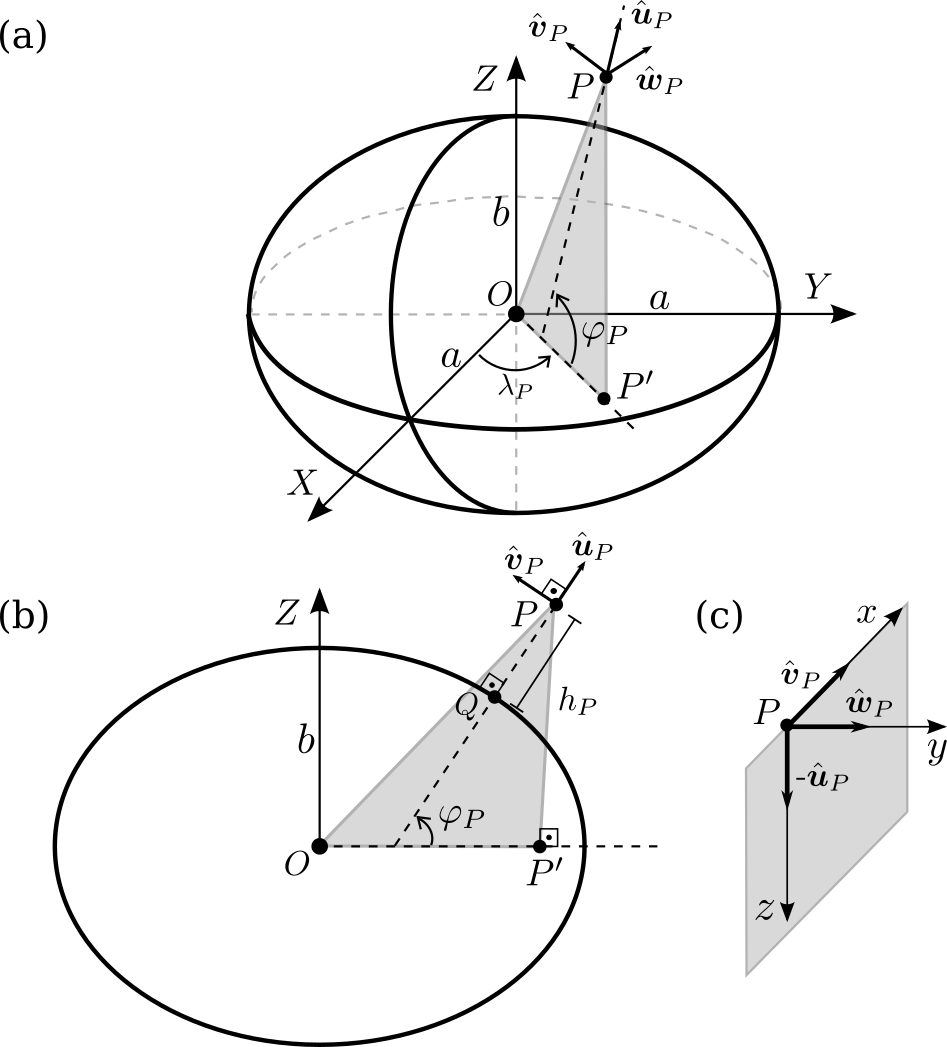
\includegraphics{figures/cartesian-geodetic-systems.png}
    \caption{Schematic representation of the Geocentric Cartesian System (GCS) and the Geocentric Geodetic System (GGS). The GCS has the $Z$-axis coincident with the mean Earth's rotational axis,
    the $X$-axis pointing to the Greenwich meridian and the $Y$-axis
    directed so as to obtain a right-handed system. The GGS is      defined by an oblate ellipsoid with semi-minor axis $b$, 
    coincident with the $Z$-axis of GCS, and a semi-major
    axis $a$. In this coordinate system, the position of a point is
    determined by the geometric height $h$, geodetic latitude 
    $\varphi$ and longitude $\lambda$. 
    The Earth's center of mass is represented 
    by $O$, $P$ represents a point $(h_{P}, \varphi_{P}, \lambda_{P})$ and $P^{\prime}$ its projection onto the plane $XY$ 
    (Equatorial plane). The plane containing $O$, $P$ and 
    $P^{\prime}$ is represented in gray in (a) and (b). 
    The unit vectors $\hat{\mitbf{u}}_{P}$, $\hat{\mitbf{v}}_{P}$ and 
    $\hat{\mitbf{w}}_{P}$ define three mutually orthogonal 
    directions at $P$ (eq. \ref{eq:unit-vectors}).
    In (b), $Q$ represents a point $(h_{Q}, \varphi_{Q}, \lambda_{Q})$,
    which is the projection of $P$ onto the reference ellipsoid, at
    the same latitude and longitude ($\varphi_{Q} = \varphi_{P}$ and $\lambda_{Q} = \lambda_{P}$).}
  \label{fig:GCS-GGS}
\end{figure}

\begin{figure}
    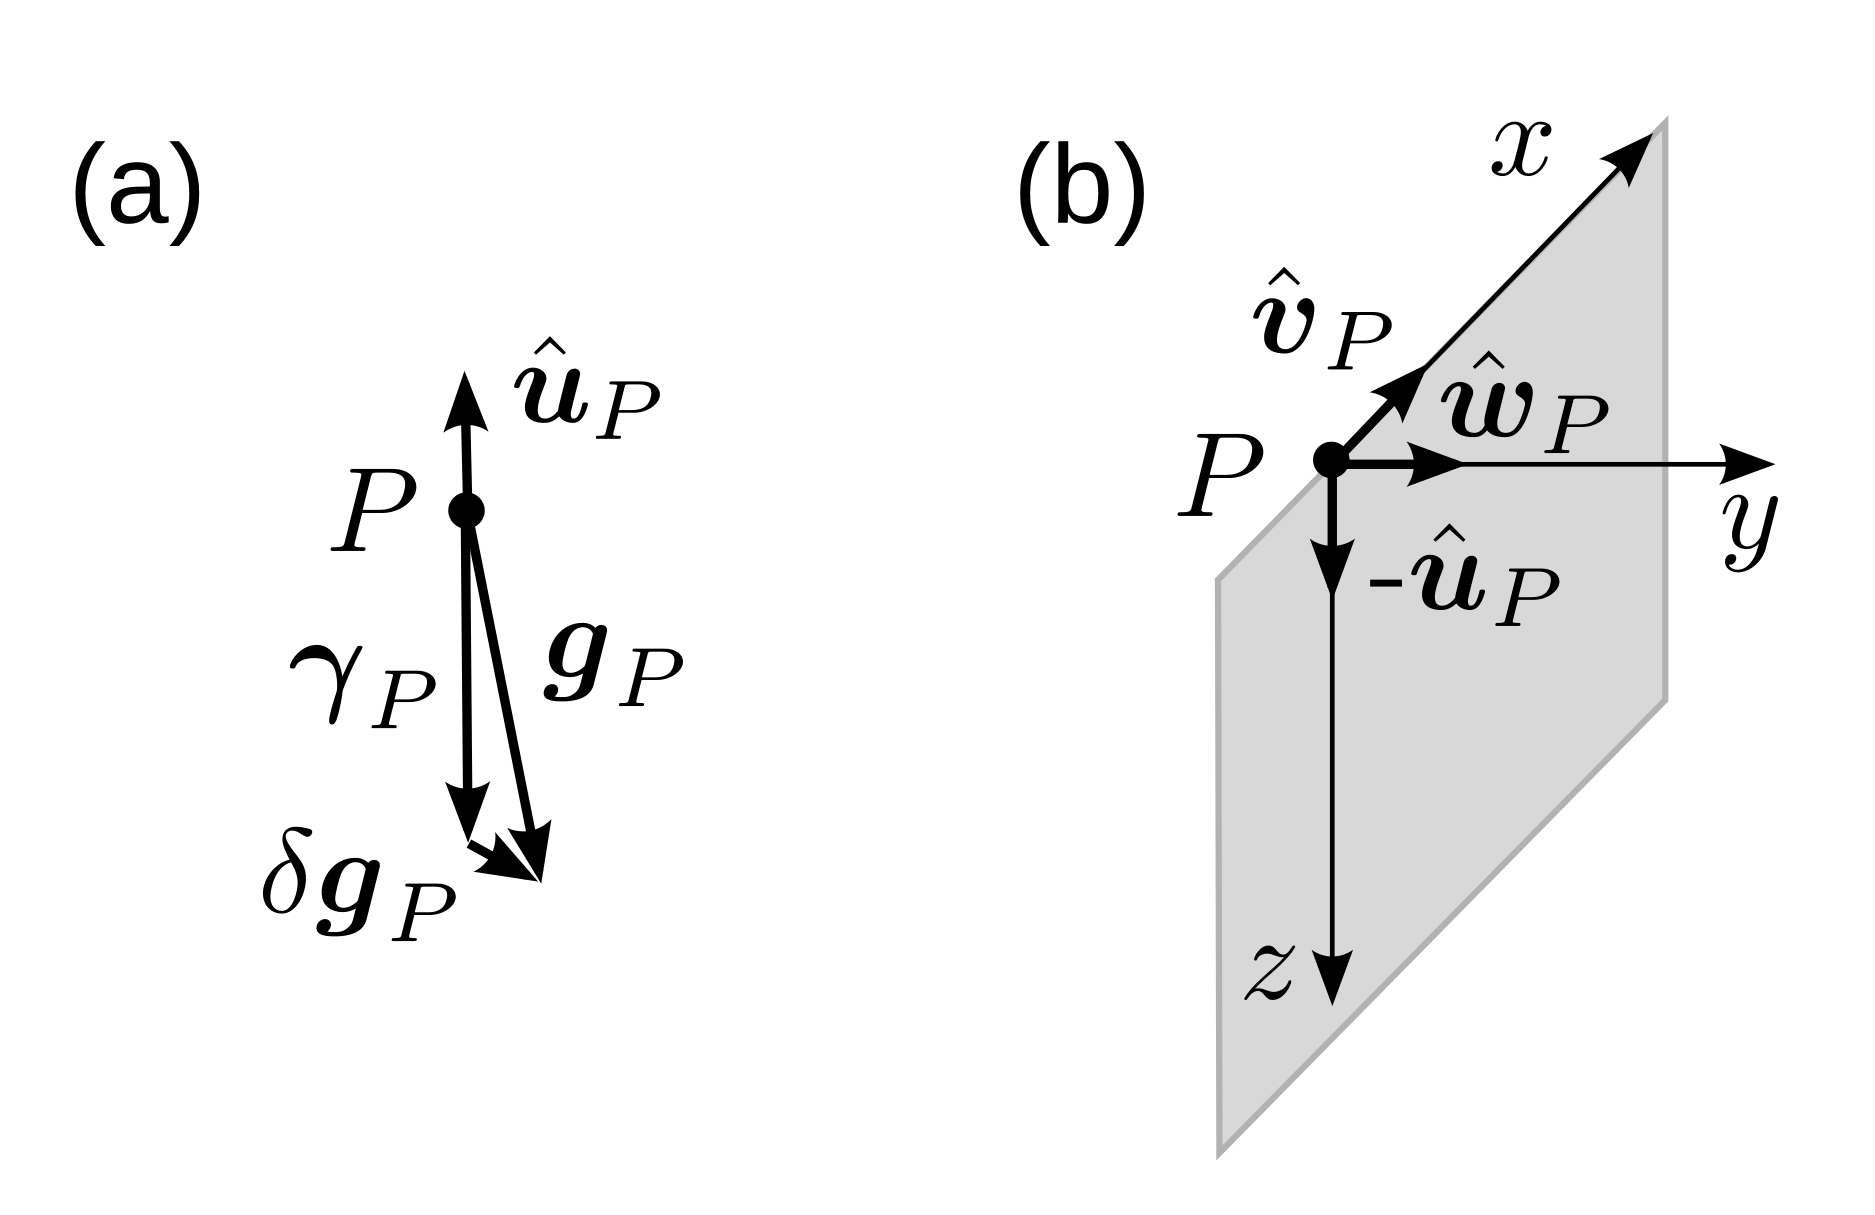
\includegraphics{figures/local-system.png}
    \caption{(a) Schematic representation of a topocentric Cartesian 
    coordinate system (TCS) with origin at a point $P$. The axes $x$
    and $y$ are parallel to the unit vectors $\hat{\mitbf{v}}_{P}$
    and $\hat{\mitbf{w}}_{P}$ (eq. \ref{eq:unit-vectors} and
    Fig. \ref{fig:GCS-GGS}), respectively. On the other hand, the $z$ axis is opposite to the unit vector $\hat{\mitbf{u}}_{P}$ (eq. 
    \ref{eq:unit-vectors} and Fig. \ref{fig:GCS-GGS}) and points downward. The gray plane is the same shown in Fig. \ref{fig:GCS-GGS}.
    (b) Schematic representation of the gravity vector
    $\mitbf{g}_{P}$, normal gravity vector $\mitbf{\gamma}_{P}$,
    gravity disturbance vector $\delta \mitbf{g}_{P}$
    (eq. \ref{eq:gravity-disturbance-vector}) and unit vector 
    $\hat{\mitbf{u}}_{P}$ (eq. \ref{eq:unit-vectors}) at a point 
    $P$.}
  \label{fig:TCS}
\end{figure}

\begin{figure}
    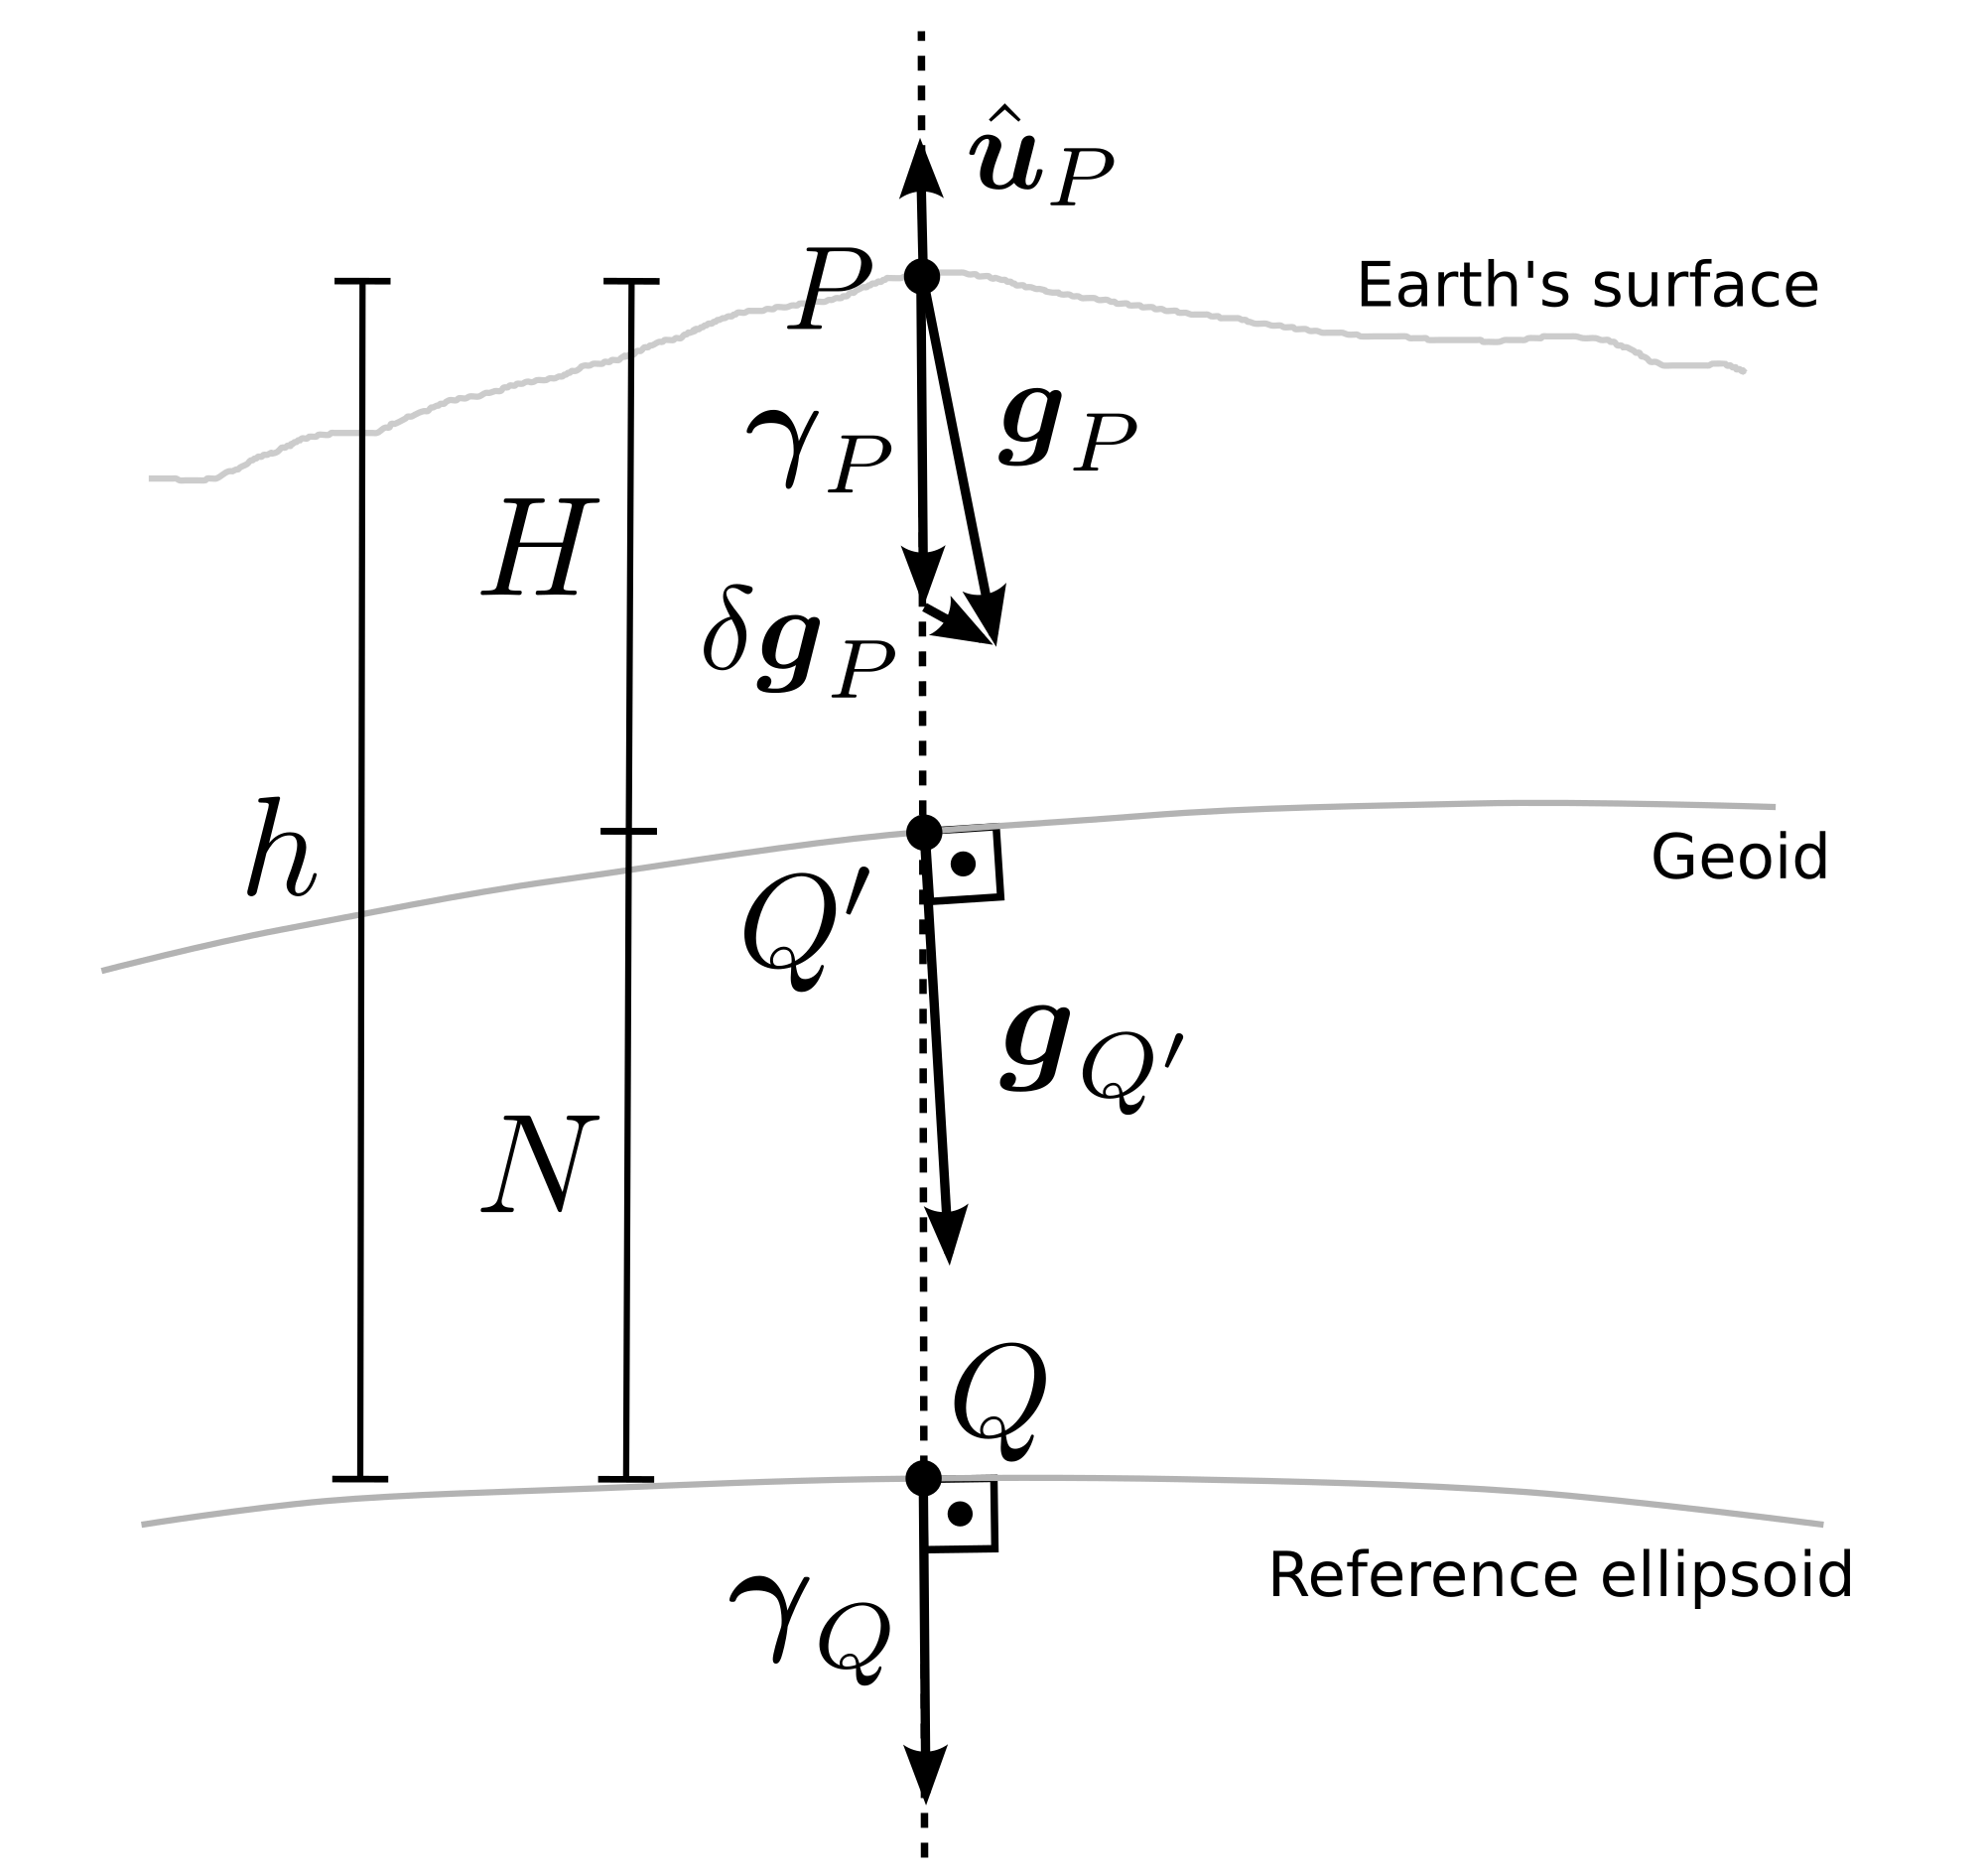
\includegraphics{figures/surfaces.png}
    \caption{Schematic representation of the gravity vector
        $\mitbf{g}_{P}$, normal gravity vector $\mitbf{\gamma}_{P}$,
        gravity disturbance vector $\delta \mitbf{g}_{P}$
        (eq. \ref{eq:gravity-disturbance-vector}), unit vector 
        $\hat{\mitbf{u}}_{P}$ (eq. \ref{eq:unit-vectors}) at a point $P$ 
        on the surface of the Earth, gravity vector $\mitbf{g}_{Q^{\prime}}$ 
        at a point $Q^{\prime}$ on the Geoid, normal gravity vector 
        $\mitbf{\gamma}_{Q}$ at a point $Q$ on the reference ellipsoid,
        geometric height $h$, orthometric height $H$ and geoidal undulation 
        $N$ \citep{heiskanen-moritz1967}.
        The dashed line passing through
        $Q$, $Q^{\prime}$ and $P$ is normal to the 
        surface of the reference ellipsoid at $Q$. This figure
        shows a commonly used approximation in which the ellipsoid 
        surface and the Geoid are represented as parallel surfaces, 
        so that $h \approx H + N$.}
  \label{fig:surfaces}
\end{figure}

\label{lastpage}


\end{document}\grid
